% bei Standalone in documentclass noch:
% \RequirePackage{luatex85}

\documentclass[captions=tableheading, titlepage= firstiscover, parskip = half , bibliography=totoc]{scrartcl}
%paper = a5 für andere optinen
% titlepage= firstiscover
% bibliography=totoc für bibdateien
% parskip=half  Veränderung um Absätze zu verbessern

\usepackage{scrhack} % nach \documentclass
\usepackage[aux]{rerunfilecheck}
\usepackage{polyglossia}
\usepackage[style=numeric, backend=biber]{biblatex} % mit [style = alphabetic oder numeric] nach polyglossia
\addbibresource{lit.bib}
\setmainlanguage{german}

\usepackage[autostyle]{csquotes}
\usepackage{amsmath} % unverzichtbare Mathe-Befehle
\usepackage{amssymb} % viele Mathe-Symbole
\usepackage{mathtools} % Erweiterungen für amsmath
\usepackage{fontspec} % nach amssymb
% muss ins document: \usefonttheme{professionalfonts} % für Beamer Präsentationen
\usepackage{longtable}

\usepackage[
math-style=ISO,    % \
bold-style=ISO,    % |
sans-style=italic, % | ISO-Standard folgen
nabla=upright,     % |
partial=upright,   % /
]{unicode-math} % "Does exactly what it says on the tin."
\setmathfont{Latin Modern Math}
% \setmathfont{Tex Gyre Pagella Math} % alternativ

\usepackage[
% die folgenden 3 nur einschalten bei documenten
locale=DE,
separate-uncertainty=true, % Immer Fehler mit ±
per-mode=symbol-or-fraction, % m/s im Text, sonst \frac
]{siunitx}

% alternativ:
% per-mode=reciprocal, % m s^{-1}
% output-decimal-marker=., % . statt , für Dezimalzahlen

\usepackage[
version=4,
math-greek=default,
text-greek=default,
]{mhchem}

\usepackage[section, below]{placeins}
\usepackage{caption} % Captions schöner machen
\usepackage{graphicx}
\usepackage{grffile}
\usepackage{subcaption}

% \usepackage{showframe} Wenn man die Ramen sehen will

\usepackage{float}
\floatplacement{figure}{htbp}
\floatplacement{table}{htbp}

\usepackage{mhchem} %chemische Symbole Beispiel: \ce{^{227}_{90}Th+}


\usepackage{booktabs}

 \usepackage{microtype}
 \usepackage{xfrac}

 \usepackage{expl3}
 \usepackage{xparse}

 % \ExplSyntaxOn
 % \NewDocumentComman \I {}  %Befehl\I definieren, keine Argumente
 % {
 %    \symup{i}              %Ergebnis von \I
 % }
 % \ExplSyntaxOff

 \usepackage{pdflscape}
 \usepackage{mleftright}

 % Mit dem mathtools-Befehl \DeclarePairedDelimiter können Befehle erzeugen werden,
 % die Symbole um Ausdrücke setzen.
 % \DeclarePairedDelimiter{\abs}{\lvert}{\rvert}
 % \DeclarePairedDelimiter{\norm}{\lVert}{\rVert}
 % in Mathe:
 %\abs{x} \abs*{\frac{1}{x}}
 %\norm{\symbf{y}}

 % Für Physik IV und Quantenmechanik
 \DeclarePairedDelimiter{\bra}{\langle}{\rvert}
 \DeclarePairedDelimiter{\ket}{\lvert}{\rangle}
 % <name> <#arguments> <left> <right> <body>
 \DeclarePairedDelimiterX{\braket}[2]{\langle}{\rangle}{
 #1 \delimsize| #2
 }

\setlength{\delimitershortfall}{-1sp}

 \usepackage{tikz}
 \usepackage{tikz-feynman}

 \usepackage{csvsimple}
 % Tabellen mit \csvautobooktabular{"file"}
 % muss in table umgebung gesetzt werden


% \multicolumn{#Spalten}{Ausrichtung}{Inhalt}

\usepackage{hyperref}
\usepackage{bookmark}
\usepackage[shortcuts]{extdash} %nach hyperref, bookmark

\newcommand{\ua}[1]{_\symup{#1}}
\newcommand{\su}[1]{\symup{#1}}


\title{Versuch 302}
\subtitle{Elektrische Brückenschaltunge}
\author{Sebastian Pape\\
        sepa@gmx.de \and
        Jonah Nitschke\\
        lejonah@web.de}
\date{Durchführung: 13.12.2016\\
      Abgabe: 20.12.2016}

\begin{document}
\maketitle
\setcounter{page}{1}
%\section{Zielsetzung}
%In diesem Versuch sollte mit Hilfe von Brückenschaltungen die physikalische Größe
%von verschieden Bauteilen bestimmt werden.
\section{Theorie}

\subsection{Elektrische Brückenschaltungen}

Bei Brückenschaltungen handelt es sich um elektrische Schaltungen, mit dessen
Hifle die Widerstände von Bauteilen sehr genau bestimmt werden können.
Hierbei sind auch komplexe Widerstände erlaubt, sodass auch die Kapazität eines
Kondestors und die Induktivität einer Spulen gemessen werden können.
Die grundlegende Struktur einer Brückenschaltung ist in Abb. \ref{fig:Brückenschaltung}
dargestellt.

\begin{figure}
  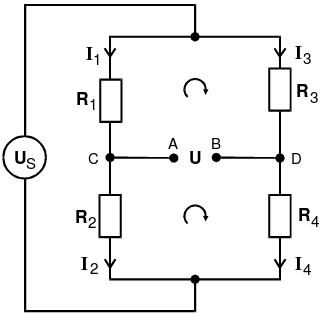
\includegraphics[width=7.50cm, height=6cm]{V302_Brückenschaltung.png}
  \caption{Grundlegende Struktur einer Brückenschaltung\cite{anleitung01}}
  \label{fig:Brückenschaltung}
\end{figure}

Es wird ausgenutzt, dass zwischen zwei getrennten stromdurchflossenen
Leitern eine Potentialdifferenz besteht, die durch die \emph{Kirchhoffschen Gesetze}
bestimmt werden kann.\\\\

1.\emph{Kirchhoffsches Gesetz} (Knotenregel):\\
Die Summe aller in ein Knoten eingehenden Ströme ist gleich der Summe, der aus
einem Knoten herausfließenden Ströme. Diese Gleichung ergibt sich aus der
Ladungserhaltung.

\begin{equation}
  \label{eqn:Kirchhoff1}
  \sum\ua{k} I\ua{k} = 0
\end{equation}

2.\emph{Kirchhoffsche Gesetz} (Maschenregel):\\
Die Summe aller Spannungen in einer Masche ist gleich Null.
Dieses Gesetzt entstammt aus der Energieerhaltung.

\begin{equation}
  \label{eqn:Krichhoff2}
  \sum\ua{k}U\ua{k} = \sum\ua{k}I\ua{k}R\ua{k}
\end{equation}

Der Zusammenhang zwischen der Brückenspannung $U$ und der Speisespannung $U\ua{S}$
ist durch folgenden Zusammenhang gegeben.

\begin{equation}
  \label{eqn:BrückenUndSpeisespannung}
  U\ua{Br} = \frac{R\ua{2}R\ua{3} - R\ua{1}R\ua{4}}{(R\ua{3} + R\ua{4})(Rua{1} + R\ua{2})}U\ua{S}
\end{equation}

Eine Brücke wird als abgeglichen bezeichnet, wenn die Brückenspannung $U\ua{Br}$ verschwindet.
Dies ist gerade der fall, wenn

\begin{equation}
  \label{eqn:abgleichbed}
  R\ua{1}R\ua{4} = R\ua{2}R\ua{3}
\end{equation}

erfüllt ist.
Diese Bedingung ist unabhängig von der Speisespannung $U\ua{S}$
und gilt somit für jede beliebige Speisespannung.

\subsection{Komplexe Wechselstromwiderstände}

Komplexe Wechselstromwiderstände treten auf, wenn Kondensatoren und oder Induktivitäten
in einer Schaltung verbaut sind. Für die Bauteile ergibt sich

\begin{equation*}
  Z\ua{R} = R, \qquad Z\ua{C} = \frac{1}{i\omega C}, \qquad Z\ua{L} = i\omega L.
\end{equation*}

Eine Komplexe Zahl besteht allgemein aus einem Realteil $X$ und einem Imaginärteil
$Y$. Also ist $Z$ insgesamt $Z = X + iY$.

Dabei ist $i$ die imaginäre Zahl und $\omega$ die Kreisfrequenz, mit der die
Spannung wechselt. Damit die Abgleichbedingung \eqref{eqn:abgleichbed} für die
Brückenschaltung für komplexe Widerstände erfüllt ist müssen der Realteil und der
Imaginärteil des Gesamtwiderstandes einzeln verschwinden. Somit ergibt sich

\begin{align}
  X\ua{1}X\ua{4} - Y\ua{1}Y\ua{4} &= X\ua{2}X\ua{3} - Y\ua{2}Y\ua{3}\label{eqn:RealteilAbgleichbed}\\
  X\ua{1}Y\ua{4} + X\ua{4}Y\ua{1} &= X\ua{2}Y\ua{3} + x\ua{3}Y\ua{3}\label{enq:ImaginärteilAbgleichbed}.
\end{align}

Dabei ist $X\ua{i}$ der Realteil und $Y\ua{i}$ der Imaginärteil.

\section{Versuchsaufbau}

In dem Versuch wurden verschiedene Brückenschaltungen verwendet. In dem folgendem
Abschnitt werden die verwendeten Schaltungen erläutert und die dazugehörigen
Formeln angegeben.

\subsection{Wheatstonesche Brücke}

Die Wheatstonesche Brücke wird für die Widerstandsmessung eines unbekannten
Widerstandes verwendet. In der Schaltung werden ausschließlich ohmsche Widerstände
verwendet.

\FloatBarrier
\begin{figure}
  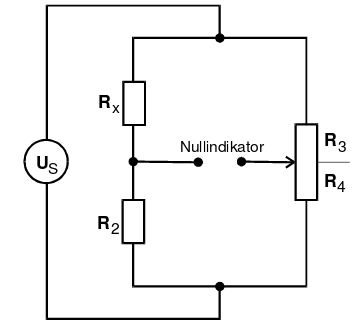
\includegraphics[width=7.50cm, height=6cm]{V302_Wheatstone.png}
  \caption{Schaltungsskizze einer Wheatstonsche Brückenchaltung\cite{anleitung01}}
  \label{fig:Wheatstone}
\end{figure}
\FloatBarrier

Der unbekannte Widerstand lässt sich mit Hilfe von \eqref{eqn:Kirchhoff1} und
\eqref{eqn:Krichhoff2} ermitteln. Es ergibt sich
\begin{equation}
  \label{eqn:Wheatstone}
  R\ua{x} = R\ua{2}\frac{R\ua{3}}{R\ua{4}}.
\end{equation}

Dabei werden $R\ua{3}$ und $R\ua{4}$so eingestellt, dass die Brücke nach
der Bedingung \eqref{eqn:abgleichbed} abgeglichen ist.

\subsection{Kapazitätsmessbrücke}

Ein idealer Kondensator kann durch ergänzen eines ohmschen Widerstandes zu einem
realen Kondensator umgewandelt werden. Ein realer Kondensator ist verlustbehaftet.
Diese Eigenschaft wird von dem ergänzten ohmschen Widerstand übernommen.
Mit Hilfe einer Kapazitätsmessbrücke kann die Kapazität und der Widerstand eines
realen Kondensators bestimmt werde.
Dafür wird der in Abb. \ref{fig:Kapazitätsmessbrücke} Aufbau verwendet.

\begin{figure}
  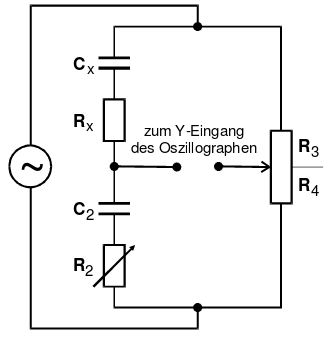
\includegraphics[width=7.50cm, height=6cm]{V302_Kapazitätsmessbrücke.png}
  \caption{Schaltungsskizze einer Kapazitätsmessbrücke\cite{anleitung01}}
  \label{fig:Kapazitätsmessbrücke}
\end{figure}

Über die Knoten- und Maschenregel ergeben sich für die unbekannten Größen
$R\ua{x}$ und $C\ua{x}$ folgende Gleichungen.

\begin{align}
  R\ua{x} &= R\ua{2}\frac{R\ua{3}}{R\ua{4}}\label{KapazitätsmessbrückeRx}\\
  C\ua{x} &= C\ua{2}\frac{R\ua{4}}{R\ua{3}}\label{KapazitätsmessbrückeLx}
\end{align}

\subsection{Induktivitätsmessbrücke}

Die Induktivitätsmessbrücke ist der Kapazitätsmessbrücke sehr ähnlich, nur anstelle
des zu bestimmenden Kondensators wird die zu vermessende Spule eingebaut.
Ebenso ist die ideal Spule mit einem ohmschen Widerstand zu versehen, sodass
die sie das Verhalten einer realen Spule beschreibt.
\begin{figure}
  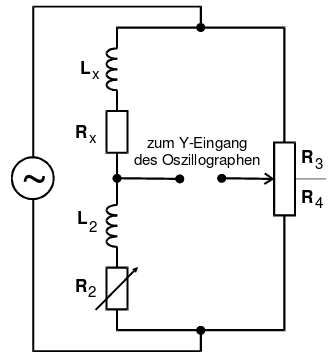
\includegraphics[width=7.50cm, height=6cm]{V302_Induktivitätsmessbrücke}
  \caption{Schaltungsskizze einer Induktivitätsmessbrücke\cite{anleitung01}}
  \label{fig:Induktivitätsmessbrücke}
\end{figure}

Durch die Komplexen Abgleichbedingungen \eqref{eqn:RealteilAbgleichbed} und
\eqref{enq:ImaginärteilAbgleichbed} ergeben sich

\begin{align}
  R\ua{x} &= R\ua{2}\frac{R\ua{3}}{R\ua{4}}\label{InduktivitätmessbrückeRx}\\
  L\ua{x} &= L\ua{2}\frac{R\ua{3}}{R\ua{4}}.\label{InduktivitätmessbrückeLx}
\end{align}

Die Induktivität und der Widerstand von einer realen Spule ist mit der
Induktivitätsmessbrücke schwierig zu vermessen. Der Wirkanteil sollte
möglichst alleine durch $R\ua{2}$ realisiert werden und $L\ua{2}$ sollte
eine möglichst hohe Effizienz haben, damit $L\ua{x}$ und $R\ua{x}$ präzise vermessen
werden können. Dies ist experimentell schwierig umzusetzen.
Deshalb wird für die Messung von Induktivitäten die Maxwell-Brücke verwendet.

\subsection{Maxwell-Brücke}

Bei der Maxwell-Brücke wird parallel zum vierten ohmsche Widerstand $R\ua{4}$
eine Kondensator mit der Kapazität $C\ua{4}$ geschaltet. Die Schaltung ist in
Abb. \ref{fig:Maxwell-Brücke} skizziert.

\begin{figure}
  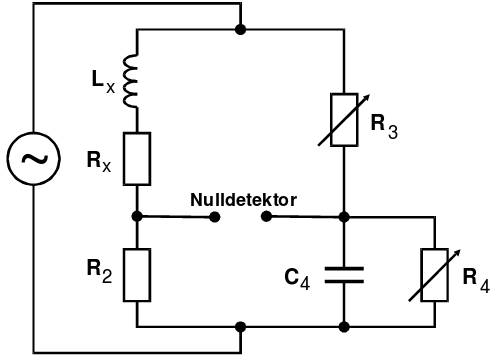
\includegraphics[width=7.50cm, height=6cm]{V302_MaxwellBrücke.png}
  \caption{Schaltungsskizze einer Maxwell-Brücke\cite{anleitung01}}
  \label{fig:Maxwell-Brücke}
\end{figure}

Durch die Komplexen Abgleichbedingungen \eqref{eqn:RealteilAbgleichbed} und
\eqref{enq:ImaginärteilAbgleichbed} ergeben sich

\begin{align}
  R\ua{x} &= \frac{R\ua{2}R\ua{3}}{R\ua{4}}\label{eqn:Maxwell_Rx}\\
  L\ua{x} &= R\ua{2}R\ua{3}C\ua{4}.\label{eqn:Maxwell_Lx}
\end{align}

Die Regelwiderstände $R\ua{3}$ und $R\ua{4}$ werden als Abgleichelemente verwendet
und der Kondensator sollte für eine präzise Messung möglichst verlustarm sein.

\subsection{Wien-Robinson-Brücke}
Die Wien-Robinson-Brücke ist eine frequenzabhängige Brückenschaltung. Der Zusammenhang
zwischen der Brückenspannung und der Speisespannung kann über die Formel
\eqref{eqn:BrückenUndSpeisespannung} berechnet werden. Für die Schaltung der
Wien-Robinson-Brücke ergibt sich die folgenden Formel.

\begin{equation}
  \label{eqn:Wien-Robinson-Brücke}
  \left|\frac{U\ua{Br}}{U\ua{S}}\right|^2 = \frac{\left(\omega^2R^2C^2 - 1\right)^2}{
  9\left[\left(1 - \omega^2R^2C^2\right)^2 + 9\omega^2R^2C^2\right]}
\end{equation}

Die Brückenspannung verschwindet für die Frequenz $\omega\ua{0} = \frac{1}{RC}$.
Somit wird die Frequenz $\omega\ua{0}$ gefiltert und alle Schwingungen mit
der Frequenz $\omega\ua{0}$ werden nicht durch diese Brückenschaltung durchgelassen.
Schwingungen mit einer Frequenz nahe von $\omega\ua{0}$ werden stark abgeschwächt.

\begin{figure}
  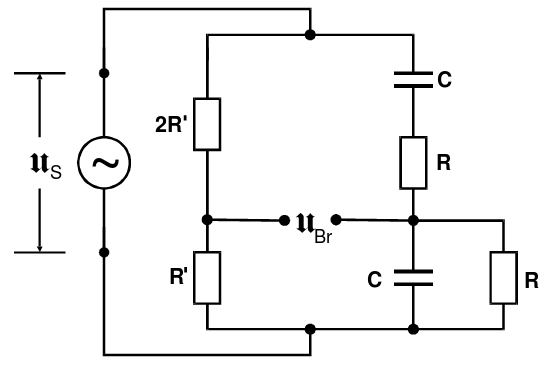
\includegraphics[width=7.50cm, height=6cm]{V302_Wien-Robinson_Brücke.png}
  \caption{Schatungsskizze einer Wien-Robinson-Brücke\cite{anleitung01}}
  \label{fig:Wien-Robinson-Brücke}
\end{figure}

\subsection{Klirrfaktor}

In dem Versuch soll der Klirrfaktor des verwendeten Sinusgenerator bestimmt werden.
Der Klirrfaktor ist eine Zeichen der Güte eines Generators und beschreibt die
Anteile der Oberwellen im Verhältnis zu der Grundwelle.
Der Klirrfaktor kann mit Hilfe der Wien-Robinson-Brücke (Abb.\ref{fig:Wien-Robinson-Brücke})
ermittelt werden. Dafür stellt man die Widerstände so ein, dass die Brückenspannung
minimal ist. An diesem Minimun ist die Frequenz $\omega\ua{0}$ erreicht, bei dem
nur noch die Oberwellen des Sinusgenerators durch die Schaltungen gelassen werden.\\
Der Klirrfaktor ist definiert als:

\begin{equation}
  \label{eqn:Klirrfaktor}
  k := \frac{\sqrt{U\ua{2}^2} + U\ua{3}^2 + ... }{U\ua{1}}.
\end{equation}

Dabei ist $U\ua{1}$ die Amplitude der Grundwelle und $U\ua{i}$ die Amplitude der
i-ten Oberwelle. Zur vereinfachten Rechnung wird hierbei lediglich $U\ua{2}$
berücksichtigt.

\section{Auswertung}

Die verwendeten Zylinder wurden mithilfe einer Schieblehre vermessen und
hatten die folgenden Längen. Dabei werden die Werte als fehlerfrei angenommen.

\begin{description}
  \item[Zylinder 1] \SI{40,35}{\milli\meter}
  \item[Zylinder 2] \SI{80,55}{\milli\meter}
  \item[Zylinder 3] \SI{80,45}{\milli\meter}
  \item[Zylinder 4] \SI{102,1}{\milli\meter}
  \item[Zylinder 5] \SI{31,1}{\milli\meter}
  \item[Zylinder 6] \SI{39,7}{\milli\meter}
  \item[Zylinder 7] \SI{61,5}{\milli\meter}
\end{description}

\subsection{Bestimmung der Dämpfungskonstante und der Schallgeschwindigkeit mit dem Impuls--Echo--Verfahren}

Die Dämpfungskonstante $\alpha$ aus \eqref{eqn:Intensität}
lässt sich aus den genommenen Daten berechnen. Dafür werden die Messdaten
in die Formel \eqref{eqn:Intensität} eingesetzt und wie folgt nach $\alpha$ aufgelöst.

\begin{equation}
  \label{eqn:dämpfung}
  \alpha = - \frac{1}{x_1} \ln{\left(\frac{I_0^\text{'}}{I_0}\right)}
\end{equation}

Dabei ist $I_0^\text{'}$ die Amplitude an der Stelle $x_1 > 0$ und $I_0$
die Amplitude an der Stelle $x  = 0$.

Die Messdaten sind in Tabelle \ref{tab:Messdaten} dargestellt.
Die Werte für Zylinder 4 und den zusammengesetzten Zylinder mit dem
achten Messwert wurden für die Berechnung der Dämpfungskonstante nicht
verwendet, weil die Peaks nur bei Verstärkug ausgemessen werden konnten.
Auf das Herausrechnen des Verstärkungsfaktors wurde der Einfachheit halber verzichtet.
Im Mittel ergibt sich die Dämpfungskontante zu:

\begin{equation}
  \alpha = \SI{21.257(301)}{\per\meter}.
\end{equation}

Der Fehler ist die Standardabweichung des Mittelwertes.
Eine Darstellung der Dämpfung in Acryl ist in dem Diagramm \ref{fig:Dämpfung}
einzusehen. Dabei sind die Messdaten der Anfangs- und Endamplituden
ebenfalls eingetragen.


\begin{figure}
  \centering
  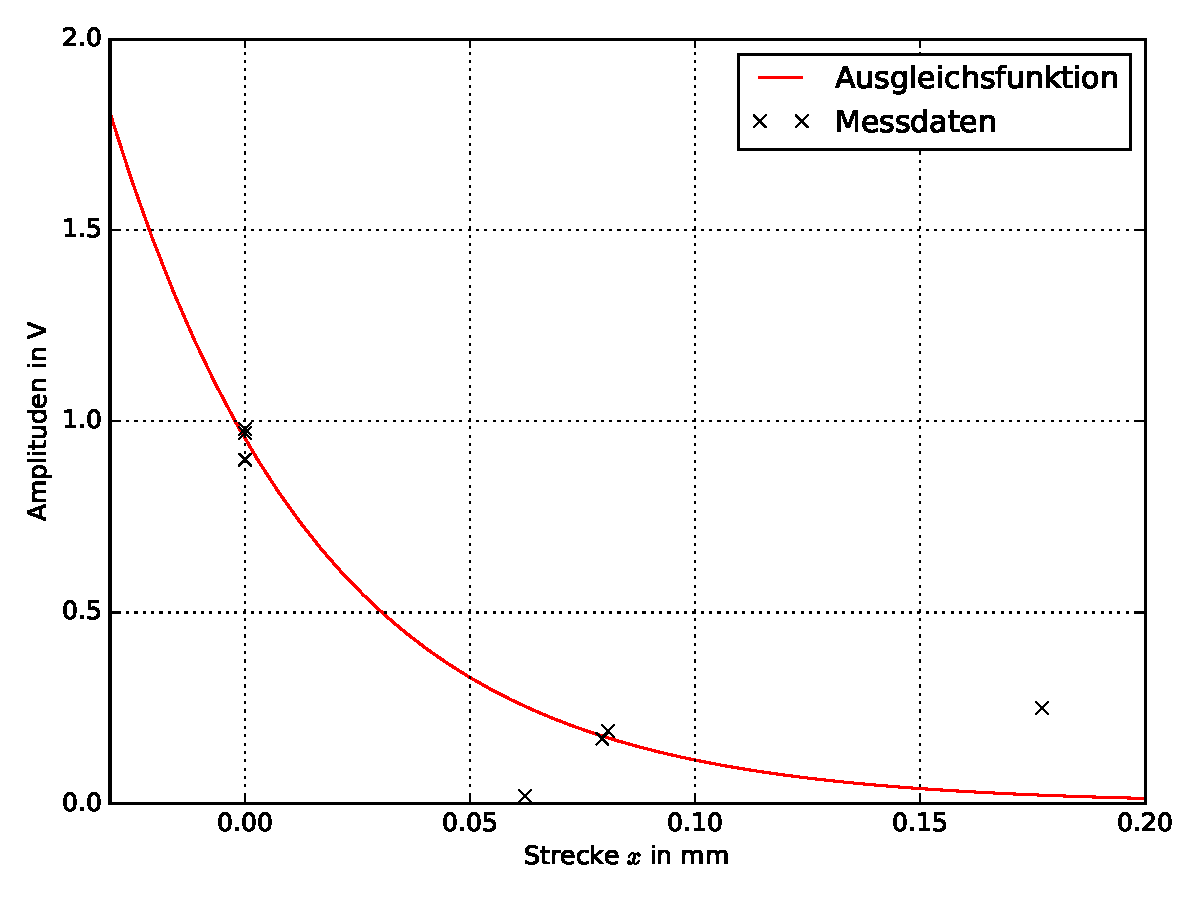
\includegraphics[width=\textwidth]{Pics/Daempfung.pdf}
  \caption{Darstellung der Dämpfung der Amplitude mit Zunahme der Strecke.}
  \label{fig:Dämpfung}
\end{figure}

Die Schallgeschwindigkeit ist aus den Laufzeiten zwischen den
gemessenen Peaks und den vermessenen Zylinderlängen mithilfe von
\eqref{eqn:Fehlstelle} zu berechnen. Dafür wurde mit dem
\emph{Python}-Packet \emph{curve\_fit} eine lineare Ausgleichsrechnung
durchgeführt. Der systematische Fehler der Sonde ist der Ordinaten-Abschnitt
der Ausgleichgeraden und die Schallgeschwindigkeit ist in der Steigung
wiederzufinden.

Die Werte ergeben sich zu:

\begin{align}
  \label{eqn:schallgesch_echo}
  c\ua{Acryl, echo} &= \SI{2880.943}{\meter\per\second} \\
  \Delta\ua{Sonde,echo} &= \SI{-3.862}{\meter\per\second}.
\end{align}

Das zugehörige Diagramm der Messung ist im Folgenden dargestellt.

\begin{figure}
  \centering
  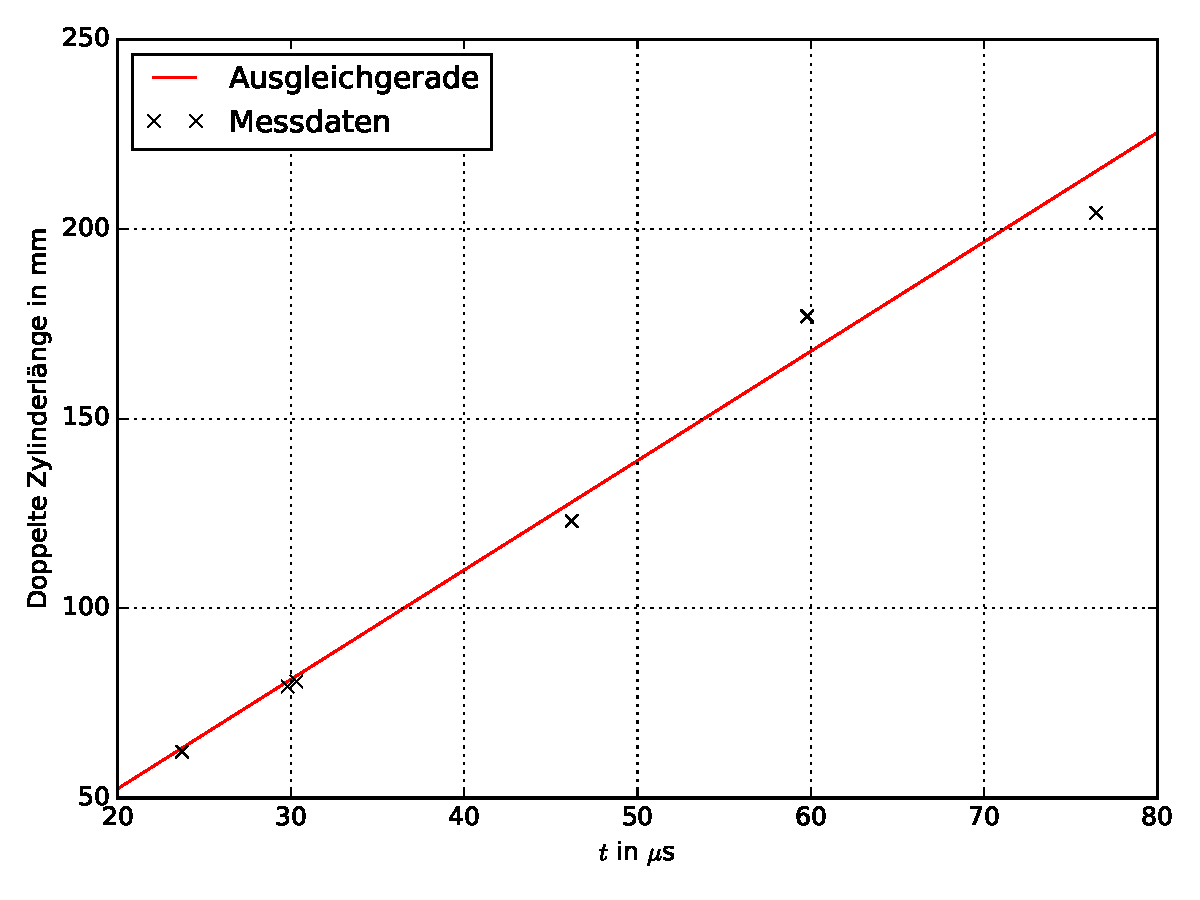
\includegraphics[width=\textwidth]{Pics/schallgesch_echo.pdf}
  \caption{Schallgeschwindigkeit in Acryl, bestimmt über das Impuls-Echo-Verfahren.}
  \label{fig:schallgesch_echo}
\end{figure}

\begin{table}
\centering
\caption{Messdaten zu dem Impuls-Echo-Verfahren. Die Werte sind den Zylindern 1 - 7 derReihe nach zuzuordnen. Der achte Messert entspricht einem Zylinder der Länge $\su{Z}_1 + \su{Z}_7$.}
\label{tab:Messdaten}
\begin{tabular}{S S S S}
\toprule
{$\su{U}\ua{1}$ in $\si{\volt}$} & {$t_1$ in $\si{\mu\second}$} & {$\su{U}\ua{2}$ in $\si{\volt}$} & {$t_2$ in $\si{\mu\second}$}  \\
\midrule
 0.90  & 0.40  & 0.17  & 30.30\\
0.97  & 0.40  & 0.02  & 59.80\\
0.98  & 0.50  & 0.01  & 59.80\\
1.00  & 0.40  & 0.12  & 76.49\\
0.97  & 0.40  & 0.25  & 23.70\\
0.98  & 0.50  & 0.19  & 29.80\\
0.97  & 0.40  & 0.04  & 46.20\\
1.00  & 0.50  & 0.12  & 75.70\\
\bottomrule
\end{tabular}
\end{table}

\FloatBarrier

\subsection{Bestimmung der Schallgeschwindigkeit mit dem Durchschallungsverfahren}

Die Messdaten zum Durchschallungsverfahren sind in Tabelle \ref{tab:durchschall}
dargestellt.
Es wurde gleich verfahren wie bei dem Impuls-Echo-Verfahren.

Die Werte ergeben sich zu:

\begin{align}
  \label{eqn:schallgesch_durch}
  c\ua{Acryl, durch} &= \SI{2878.377}{\meter\per\second} \\
  \Delta\ua{Sonde, durch} &= \SI{-2.946}{\meter\per\second}.
\end{align}

Das zugehörige Diagramm der Messung ist im Folgenden dargestellt.

\begin{figure}
  \centering
  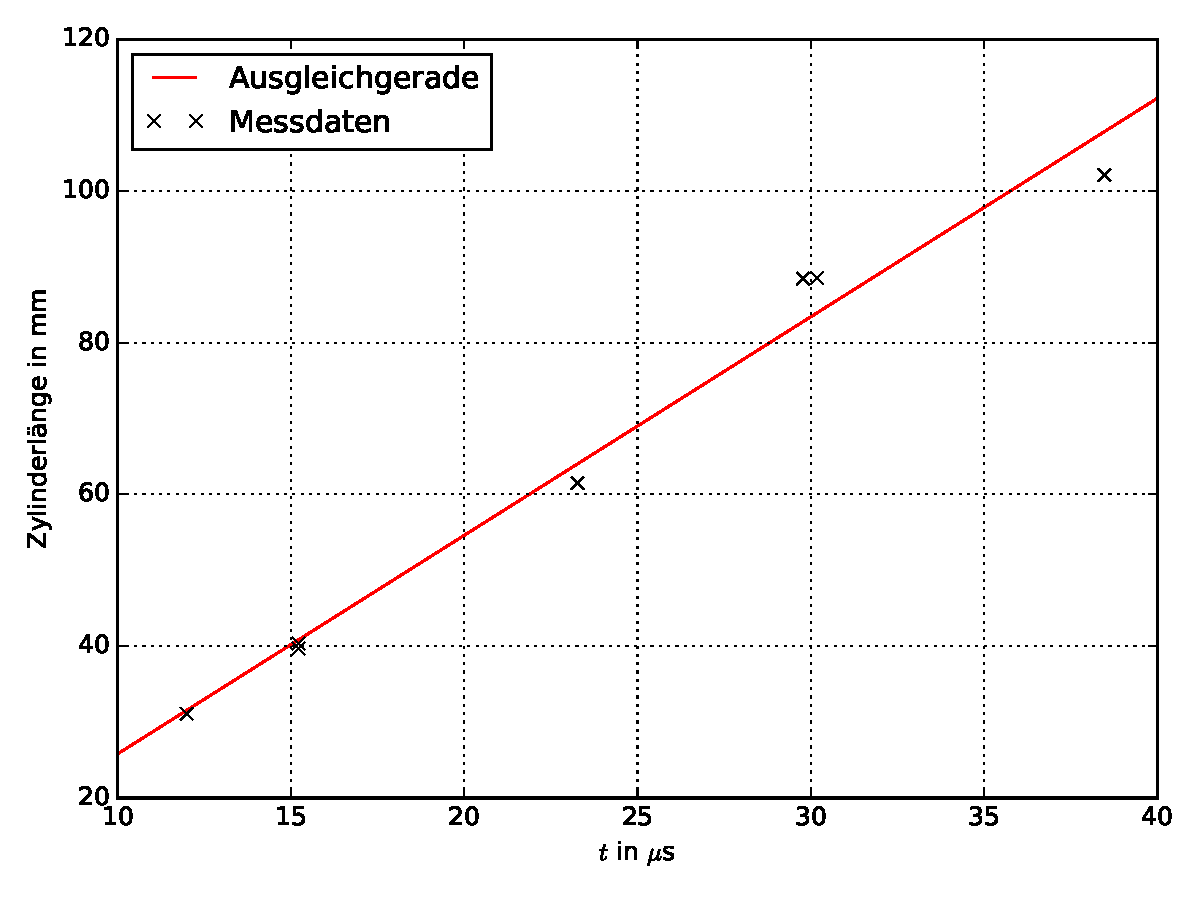
\includegraphics[width=\textwidth]{Pics/schallgesch_durch.pdf}
  \caption{Schallgeschwindigkeit in Acryl, bestimmt über das Durchschallungsverfahren.}
  \label{fig:schallgesch_durch}
\end{figure}

\begin{table}
\centering
\caption{Messdaten zu dem Durchschallungsverfahren. Die Messdaten sind der Reihe nach den Zylindern 1 - 7 zuzuordnen.}
\label{tab:durchschall}
\begin{tabular}{S }
\toprule
{Laufzeiten in \si{\mu\second}}  \\
\midrule
 15.21\\
29.78\\
30.18\\
38.48\\
11.98\\
15.21\\
23.27\\
\bottomrule
\end{tabular}
\end{table}

\FloatBarrier

\subsection{Spektrale Analyse und Cepstrum}

Die verwendeten Acrylplatten wurde mit einer Schieblehre vermessen.
Die Dicken wurden ebenfalls als fehlerfrei angenommen.

\begin{description}
  \item[Platte 1] $d_1 = \SI{9.9}{\milli\meter}$
  \item[Platte 2] $d_2 = \SI{6}{\milli\meter}$
\end{description}

Das Durchschallungsverfahren ergab die folgenden Werte.

\begin{description}
  \item[Platte 1] $d_1 = \SI{10.51}{\milli\meter}$
  \item[Platte 2] $d_2 = \SI{6.48}{\milli\meter}$
\end{description}

Die bestimmten Werte weichen um $\Delta\ua{Platte 1} = \SI{0.61}{\milli\meter}$
und $\Delta\ua{Platte 2} = \SI{0.48}{\milli\meter}$ von den mit der
Schieblehre vermessenen Werten ab.

Die Fehler aus dem systematische Fehler der Sonde sind vernachlässigbar klein.

Das Spektrum und das Cepstrum wurden aufgenommen. Die genommenen
Diagramme sind im Folgendem dargestellt.

\begin
{figure}
\centering
\begin{subfigure}{0.48\textwidth}
\centering
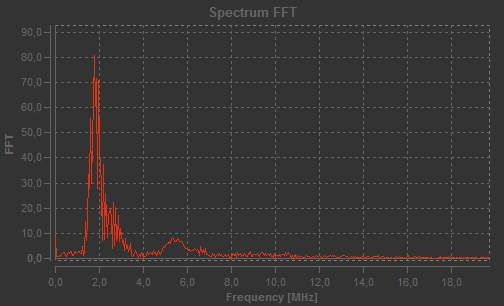
\includegraphics[height=4.2cm]{Pics/Z6_M3_S.jpg}
\caption{Aufgenommenes Spektrum.}
\label{fig:Spektrum}
\end{subfigure}
\begin
{subfigure}{0.48\textwidth}
\centering
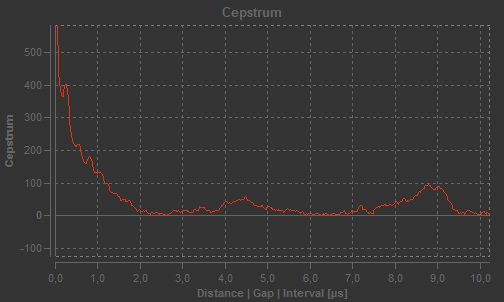
\includegraphics
[height=4.2cm]{Pics/Z6_M3_C.jpg}
\caption{Aufgenommenes Cepstrum.}
\label{fig:Cepstrum}
\end{subfigure}
\end{figure}

\subsection{Biometrische Untersuchung eines Augenmodells}

Es wurde ein Auge wie aus Abb. \ref{fig:Auge} untersucht.
Insgesamt wurden fünf Peaks aufgenommen die den folgenden Bestandteilen des Auges
zuzuordnen sind.

\begin{enumerate}
  \item Hornhaut
  \item Iris
  \item Linseneingang
  \item Linsenausgang
  \item Retina
\end{enumerate}

Die Peaks spiegeln der Aufzählung entsprechend die Bestandteilen des Auges wieder.
Für die Bereiche zwischen Hornhaut und Linseneingang, sowie
Linsenausgang und Retina wurde die Schallgeschwindigkeit für
Glaskörper verwendet ($c\ua{Glaskoerper} = \SI{1410}{\meter\per\second}$
\cite{anleitung01}).
Für den Bereich zwischen Linseneingang und Linsenausgang
wurde eine Schallgeschwindigkeit von $c\ua{Linse} = \SI{2500}{\meter\per\second}$
angenommen.

Die Bestandteile des Auges haben die folgenden Tiefen.

\begin{description}
  \item[Hornhaut] $\SI{0}{\milli\meter}$
  \item[Iris] $\SI{4.385(11)}{\milli\meter}$
  \item[Linseneingang] $\SI{7.635(18)}{\milli\meter}$
  \item[Linsenausgang] $\SI{14.835(21)}{\milli\meter}$
  \item[Retina] $\SI{44.23(9)}{\milli\meter}$
\end{description}

Die dazugehörigen Fehler entstehen durch den systematischen Fehler der Sonde.

Die Messdaten sind in der Tabelle \ref{tab:Auge} einzusehen.

\begin{table}
\centering
\caption{Messdaten zur biometrischen Untersuchung des Auges. Die Messdaten sind der Reihe den Bestandteile des Auges zuzuordnen.}
\label{tab:Auge} 
\begin{tabular}{S S }
\toprule
{Peakabstand $\Delta_{\symup{peak}}$ in \si{\mu\second}}  & {Absoluter Abstand}  \\
\midrule
 0.20  & 0.20\\
6.22  & 6.64\\
4.61  & 11.05\\
5.76  & 16.81\\
41.70  & 70.26\\
\bottomrule
\end{tabular}
\end{table}


\section{Diskussion}

Als Literaturwert der Schallgeschwindigkeit in Acryl wurde
$c\ua{Acyl, lit} = \SI{2730}{\meter\per\second}$\cite{lit} angenommen.
Die Schallgeschwindigkeit in Acryl wurde über zwei verschiedenen
Ultraschallverfahren ermittelt. Die berechneten Werte unterscheiden sich
um $\Delta\ua{c, gemessen} = \SI{1.740(917)}{\meter\per\second}$.
Hingegen liegt der Unterschied des gemittelten Wertes zum Literaturwert bei $\SI{149.246(3404)}{\meter\per\second}$.
Da beide Verfahren einen deutlichen Unterschied zu dem Literaturwert aufweisen,
aber untereinander kaum verschieden sind, wird
ein weiterer systematischer Fehler, der von dem systematischen Fehler der
Sonde verschieden ist angenommen.
Die Dicke der Acrylplatten wurden einmal über eine Schieblehre und
zum anderen über das Durchschallungsverfahren ermittelt.
Die Dicken, die sich aus dem Durchschallungsverfahren ergeben, sind
ca. einen halben Millimeter größer als die ausgemessenen Werte.
Mit dem Literaturwert für die Schallgeschwindigkeit von Acryl
ergeben sich die Plattendicken zu:

\begin{description}
  \item[Platte 1] $d_1 = \SI{9.96}{\milli\meter}$
  \item[Platte 2] $d_2 = \SI{6.14}{\milli\meter}$.
\end{description}

Damit ist die Abweichung der Plattendicken auf den systematischen Fehler
der Schallgeschwindigkeit zurückzuführen.

Die Diagramme aus der Spektralen Analyse (\ref{fig:Spektrum}, \ref{fig:Cepstrum})
werden im Folgenden diskutiert. In dem Diagramm des Cepstrums sind nicht die Lagen der tatsächlich
beobachteten Peaks erkenntlich, hingegen werden Peaks dargestellt, die
nicht beobachtet wurden. Das Spektrum zeigt einen Peak bei ca. $\SI{1.8}{\mega\hertz}$.
Die Eingangsfrequenz betrug hingegen $\SI{2}{\mega\hertz}$. Die weiteren Peaks
sind durch Reflexionen der Eingangswelle zu erklären.

Die biometrische Untersuchung des Auges ergab Werte, die
mit den Erwartungswerten übereinstimmen. Hierbei muss der
systematische Fehler ebenfalls bedacht werden, weshalb davon auszugehen
ist, dass die tatsächlichen Werte kleiner als die bestimmten Werte sind.


\printbibliography

\end{document}
